%%%%%%%%%%%%%%%%%%%%%%%%%%%%%%%%%%%%%%%%%%%%%%%%%%%%%%%%%%%%%%%%
%                                                              %
%      sPHENIX Technical Design Report at CD2 -- 2019          %
%             open for writing 2019.02.01
%             deadline to complete 2019.03.11
%                                                              %
%%%%%%%%%%%%%%%%%%%%%%%%%%%%%%%%%%%%%%%%%%%%%%%%%%%%%%%%%%%%%%%%

%%  sPHENIX TDR Editor: John Haggerty (haggerty@bnl.gov)

                           
\documentclass[12pt,twoside]{article}

%%%%%%%%%%%%%%%%
% Adding the include only list allows you to typeset only your
% chapter while maintaining overall page numbers and references.
% It also shields you from errors in other chapters as you go along.
% You need to typeset the whole thing once though. 

%\includeonly{title_page,daq_trig/daq_trig}

%%%%%%%%%%%%%%%%%%  header  (packages, 
%%%%%% Header for sPHENIX Conceptual Design Report -- 2017 

\RequirePackage{lineno}
\usepackage{import}
%\usepackage{titlesec}
\usepackage{enumitem}
\usepackage{amssymb, amsmath}
\usepackage{mathpazo}
\usepackage{float,graphicx}
%\graphicspath{{./}{pCDR/}}
\usepackage[figuresright]{rotating}
\usepackage{wrapfig}
\usepackage[usenames,dvipsnames]{color}
\usepackage{microtype}
\usepackage{tabulary}
%\usepackage{booktabs,multirow,dcolumn,bigdelim}
\newcommand{\otoprule}{\midrule[\heavyrulewidth]}
\usepackage{xr-hyper}
\usepackage[pdftex,plainpages=false,pdfpagelabels,backref,pdfborder={0 0 0}]{hyperref}
%\usepackage{hyperref}
\usepackage{url}
\usepackage[toc,page,titletoc]{appendix}
%\usepackage{afterpage}
\usepackage[font=small,labelfont=bf]{caption}
\setlength\captionmargin{15pt}
\usepackage[scaled]{helvet}
\usepackage{sectsty}
\allsectionsfont{\normalfont\sffamily}
%\usepackage{titletoc}
\usepackage{bytefield}
\usepackage{verbatimbox}
%\titlecontents{chapter}
%  [1.5em]
%  {\linespread{0.9}\normalfont\sffamily\bfseries}
%  {\contentslabel{1em}} 
%  {\hspace*{-1.3em}} 
%  {\mdseries\titlerule*[1pc]{.}\contentspage} 
%\titlecontents{section}
%  [3.5em]
%  {\linespread{0.9}\normalfont\sffamily}
%  {\contentslabel{2.3em}} 
%  {\hspace*{-2.3em}} 
%  {\titlerule*[1pc]{.}\contentspage} 
%\titlecontents{subsection}
%  [4.5em]
%  {\linespread{0.9}\normalfont\sffamily}
%  {\contentslabel{2.3em}} 
%  {\hspace*{-2.3em}} 
%  {\titlerule*[1pc]{.}\contentspage} 
%\titlecontents{subsubsection}
%  [5.5em]
%  {\linespread{0.9}\normalfont\sffamily}
%  {\contentslabel{2.3em}} 
%  {\hspace*{-2.3em}} 
%  {\titlerule*[1pc]{.}\contentspage} 
%\tolerance = 10000

\usepackage[text={6.5in,8.75in},headheight=26pt,centering]{geometry}
\usepackage{xspace}

\DeclareGraphicsExtensions{.pdf,.png}
\newcommand{\filenamedot}{.}
\setlength{\parindent}{0.0in}
\setlength{\parskip}{0.1in}
\renewcommand{\topfraction} {0.9}
\renewcommand{\bottomfraction} {0.9}
\renewcommand{\textfraction} {0.1}
\renewcommand{\floatpagefraction} {0.8}

%\usepackage{fancyhdr}
%\pagestyle{fancy}
%\renewcommand{\chaptermark}[1]{\markboth{#1}{}}
%\renewcommand{\sectionmark}[1]{\markright{#1}{}}
%\fancyhead{} % clear all header fields 
%\fancyhead[RO,LE]{\sffamily \rightmark}
%\fancyhead[LO,RE]{\sffamily \leftmark}
%\fancyfoot{} % clear all footer fields 
%\fancyfoot[RO,LE]{\sffamily \thepage}
%\renewcommand{\headrulewidth}{0pt} 
%\fancypagestyle{plain}{%
%  \fancyhf{}
%  \fancyfoot[RO,LE]{\sffamily \thepage}
%}

\usepackage{multirow}
\usepackage{eurosym}
\usepackage{xcolor}
\usepackage{framed}
\colorlet{shadecolor}{blue!10}

\usepackage{gensymb}

\setcounter{secnumdepth}{3}
\setcounter{tocdepth}{1}

\newcommand{\martinimusic}{\mbox{\sc Martini+Music}\xspace}
\newcommand{\hic}{\mbox{$A$$+$$A$}\xspace}
\newcommand{\pA}{\mbox{$p$$+$$A$}\xspace}
\newcommand{\AuAu}{\mbox{Au$+$Au}\xspace}
\newcommand{\auau}{\mbox{Au$+$Au}\xspace} 
\newcommand{\raa}{\mbox{$R_\mathrm{AA}$}\xspace}
\newcommand{\pbpb}{\mbox{Pb$+$Pb}\xspace} 
\newcommand{\pdau}{\mbox{$p(d)$$+$Au}\xspace} 
\newcommand{\pau}{\mbox{$p$$+$Au}\xspace} 
\newcommand{\aj}{\mbox{$A_J$}\xspace} 
\newcommand {\pp}{\mbox{$p$$+$$p$}\xspace}
\newcommand {\ppbar}{\mbox{$p$$+$$\overline{p}$}\xspace}
\newcommand{\pT}{\mbox{${p_T}$}\xspace}
\newcommand{\jpsi}{\mbox{$J/\psi$}}
\newcommand{\sqrtsnn}{\mbox{$\sqrt{s_{\scriptscriptstyle NN}}$}}
\newcommand{\npart}{$N_\mathrm{part}$}
\newcommand{\ncoll}{$N_\mathrm{coll}$}
\newcommand{\qgp}{\mbox{quark-gluon plasma}\xspace}
\newcommand{\jt}{\mbox{$J_T$}} \newcommand{\qhat}{\mbox{$\hat{q}$}}
\newcommand{\Qsqr}{\mbox{$Q^2$}} \newcommand{\CuCu}{\mbox{Cu$+$Cu}}
\newcommand{\PbPb}{\mbox{Pb$+$Pb}} \newcommand{\pPb}{\mbox{$p$$+$Pb}}
\newcommand{\gjet}{\mbox{$\gamma$-jet}}
\newcommand{\Qmax}{\mbox{$Q_{\max}$}} \newcommand{\ET}{\mbox{$E_T$}}
\newcommand{\Et}{\mbox{$E_T$}} \newcommand{\kt}{\mbox{$k_T$}}
\newcommand{\RAA}{\mbox{$R_{AA}$}\xspace} \newcommand{\IAA}{\mbox{$I_{AA}$}}
\newcommand{\pt}{\mbox{${p_T}$}\xspace}
\newcommand{\highpt}{high-${\rm p_{_{T}}}$}
\newcommand{\lessim}{{\stackrel{<}{\sim}}} \newcommand{\eqnpt}{p_T}
\newcommand{\eA}{\mbox{$e-{\rm A}$}}
\newcommand{\dAu}{\mbox{$d$$+$Au}\xspace}
\newcommand{\pAu}{\mbox{$p$$+$Au}\xspace}
\newcommand{\GeVSQ}{\mbox{${\rm GeV}^2$}}
\newcommand{\fastjet}{\mbox{\sc FastJet}\xspace}
\newcommand{\geant}{\mbox{\sc Geant4}\xspace}
\newcommand{\antikt}{\mbox{anti-$k_T$}\xspace}
\newcommand{\pythia}{\mbox{\sc Pythia}\xspace}
\newcommand{\opera}{\mbox{\sc Opera}\xspace}
\newcommand{\rapgap}{\mbox{\sc Rapgap}\xspace}
\newcommand{\milou}{\mbox{\sc Milou}\xspace}
\newcommand{\pyquen}{\mbox{\sc Pyquen}\xspace}
\newcommand{\hijing}{\mbox{\sc Hijing}\xspace}
\newcommand{\roofit}{\mbox{\sc RooFit}\xspace}
\newcommand{\roounfold}{\mbox{\sc RooUnfold}\xspace}
\newcommand{\beetle}{\mbox{\sc Beetle}\xspace}
\newcommand{\gj}{\mbox{$\gamma$+jet}\xspace}
\newcommand{\gh}{\mbox{$\gamma$+hadron}\xspace}
\newcommand{\martini}{\mbox{\sc Martini}\xspace}
\newcommand{\music}{\mbox{\sc Music}\xspace}
\newcommand{\Ephenix}{Electron-Ion Collider (EIC) detector built
 around the BaBar magnet and sPHENIX calorimetry\xspace}
\newcommand{\ephenix}{EIC detector built around the BaBar magnet and
 sPHENIX calorimetry\xspace} 
\newcommand{\refdesign}{reference design\xspace}
\newcommand{\refconfig}{reference configuration\xspace}
\newcommand{\dijet}{\mbox{dijet}\xspace}
\newcommand{\fake}{\mbox{fake}\xspace}
\newcommand{\fast}{\mbox{fast}\xspace}
\newcommand{\veryfast}{\mbox{very fast}\xspace}
\newcommand{\epem}{\mbox{$e^+e^-$}\xspace}
\newcommand{\onewidth}{0.6\linewidth}
\newcommand{\twowidth}{0.48\linewidth}
\newcommand{\threewidth}{0.32\linewidth}
\newcommand{\egoing}{\mbox{electron-going}\xspace}
\newcommand{\hgoing}{\mbox{hadron-going}\xspace}
\newcommand{\egodir}{electron-going direction\xspace}
\newcommand{\hgodir}{hadron-going direction\xspace}

\newcommand{\red}{\color{red}}
\newcommand{\blue}{\color{blue}}	 
\newcommand{\green}{\color{green}}	 
\newcommand{\magenta}{\color{magenta}}

\newcommand{\lyxdot}{.}
\usepackage{subcaption}

\setlength\fboxsep{0pt}
\setlength\fboxrule{0.5pt}

\usepackage[textwidth=1in,textsize=footnotesize,disable]{todonotes}
%\usepackage[textwidth=1in,textsize=footnotesize]{todonotes}

 \author[1]{Friederike Bock}
 \author[1]{Raymond Ehlers}
 \author[1]{Constantin Loizides}
 \author[2]{Tristan Protzman}
 \author[2]{Rosi J. Reed}
 \author[1]{Nicolas Schmidt}
 
 \affil[1]{Oak Ridge National Laboratory}
 \affil[2]{Lehigh University}
\begin{document}
\linenumbers
%\frontmatter
\pagestyle{empty}

%%%%%%%%%%%%%%%%%%%%%%%%%%%%%%%%% title page
\renewcommand*\familydefault{\sfdefault}
{\sffamily
\vfill
\vspace{4cm}
\begin{figure}[H]
  \begin{center}
  
\includegraphics[width=0.3\linewidth]{figs/ecce-logo.png}
\end{center}
\end{figure}

\begin{center}
  \large
  {\LARGE{ECCE Jet Resolution}}

  \begin{tabular}{cc}
&A full-acceptance detector at the EIC based on the BaBAR magnet \\
&December 1, 2021 \\
  \end{tabular}
  \end{center}

\vspace{1cm}

\begin{figure}[H]
  \begin{center}
    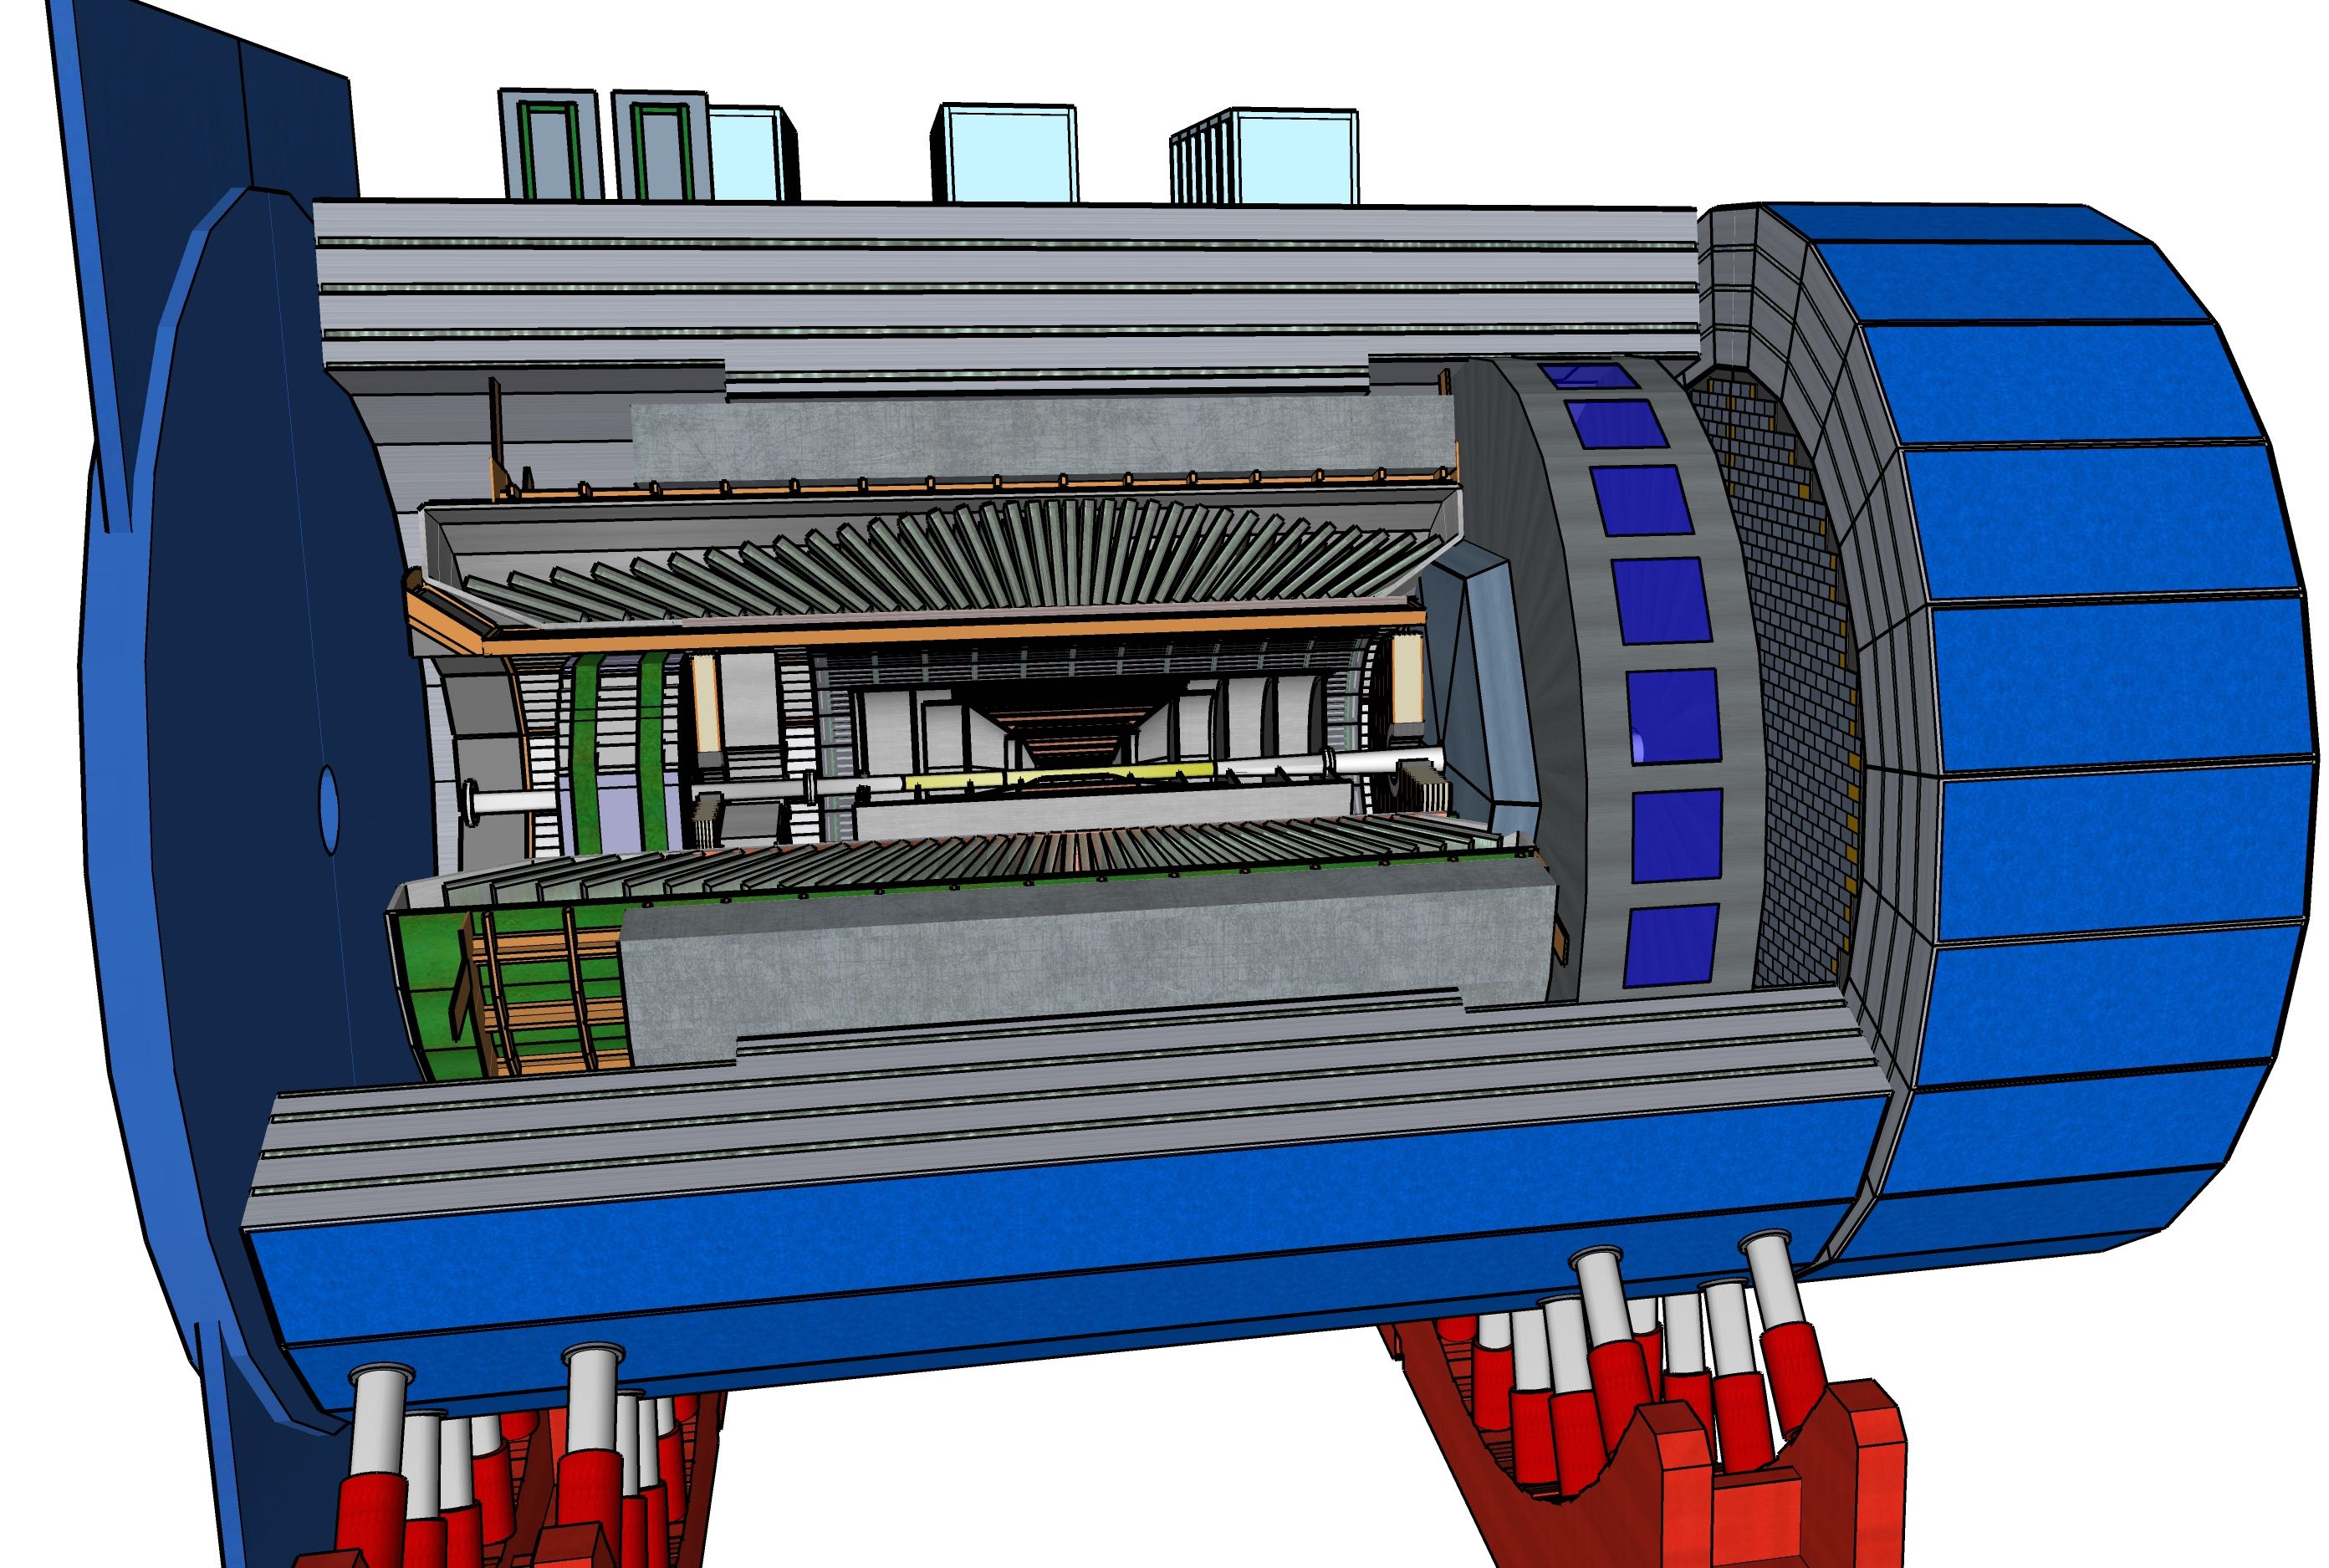
\includegraphics[width=0.7\linewidth]{figs/ECCE.png}
  \end{center}
\end{figure}
}


\vfill
\renewcommand*\familydefault{\rmdefault}

%  \author[1]{Friederike Bock}
 \author[1]{Raymond Ehlers}
 \author[1]{Constantin Loizides}
 \author[2]{Tristan Protzman}
 \author[2]{Rosi J. Reed}
 \author[1]{Nicolas Schmidt}
 
 \affil[1]{Oak Ridge National Laboratory}
 \affil[2]{Lehigh University}
%\cleardoublepage
\pagestyle{plain}

\setcounter{page}{1}

%\clearpage
%\cleardoublepage

%\resetlinenumber

\tableofcontents
%\cleardoublepage

%\mainmatter

\renewcommand{\thepage}{\arabic{page}}
%\setcounter{chapter}{0}
%\setcounter{page}{1}

\section {Introduction}
\label{det_overview}

During the hadronization process, many of the final state particles are grouped together into structures known as jets.  From these jets, the parton kinematics are able to be studied in greater detail than available from the measurement of individual particles.  Additionally, jets can yield insight into the hadronization process by studying the distribution of energy throughout a jet \cite{AbdulKhalek:2021gbh}.  Thus, it is important to know the resolution and scale which ECCE can measure jets.  
\section {Track Jets}
\label{section2}

The tracking systems of ECCE allow for the measurement of lower momentum charged jets with excellent scale and resolution.  The analysis was completed with 18x275 GeV Pythia 8 electron proton collisions, requiring a $Q^2$ greater than $100 \hbox{ GeV}^2$, and the prop.4 detector configuration.  The anti-$k_T$ jet finding algorithm was utilized, with a jet radius $R=0.5$.  To prevent the classification of single particles as jets, a constraint of $z<0.95$ as applied, where 
\begin{equation}
z=\frac{E_{\hbox{most energetic constituent}}}{E_{\hbox{total jet}}}.
\label{eq:jet_z}
\end{equation}

Jets with a transverse momentum of $p_T > 30\hbox{ GeV/c}$ are rejected to stay within the limits of the tracking detectors.

\begin{figure}[h]
    \centering
    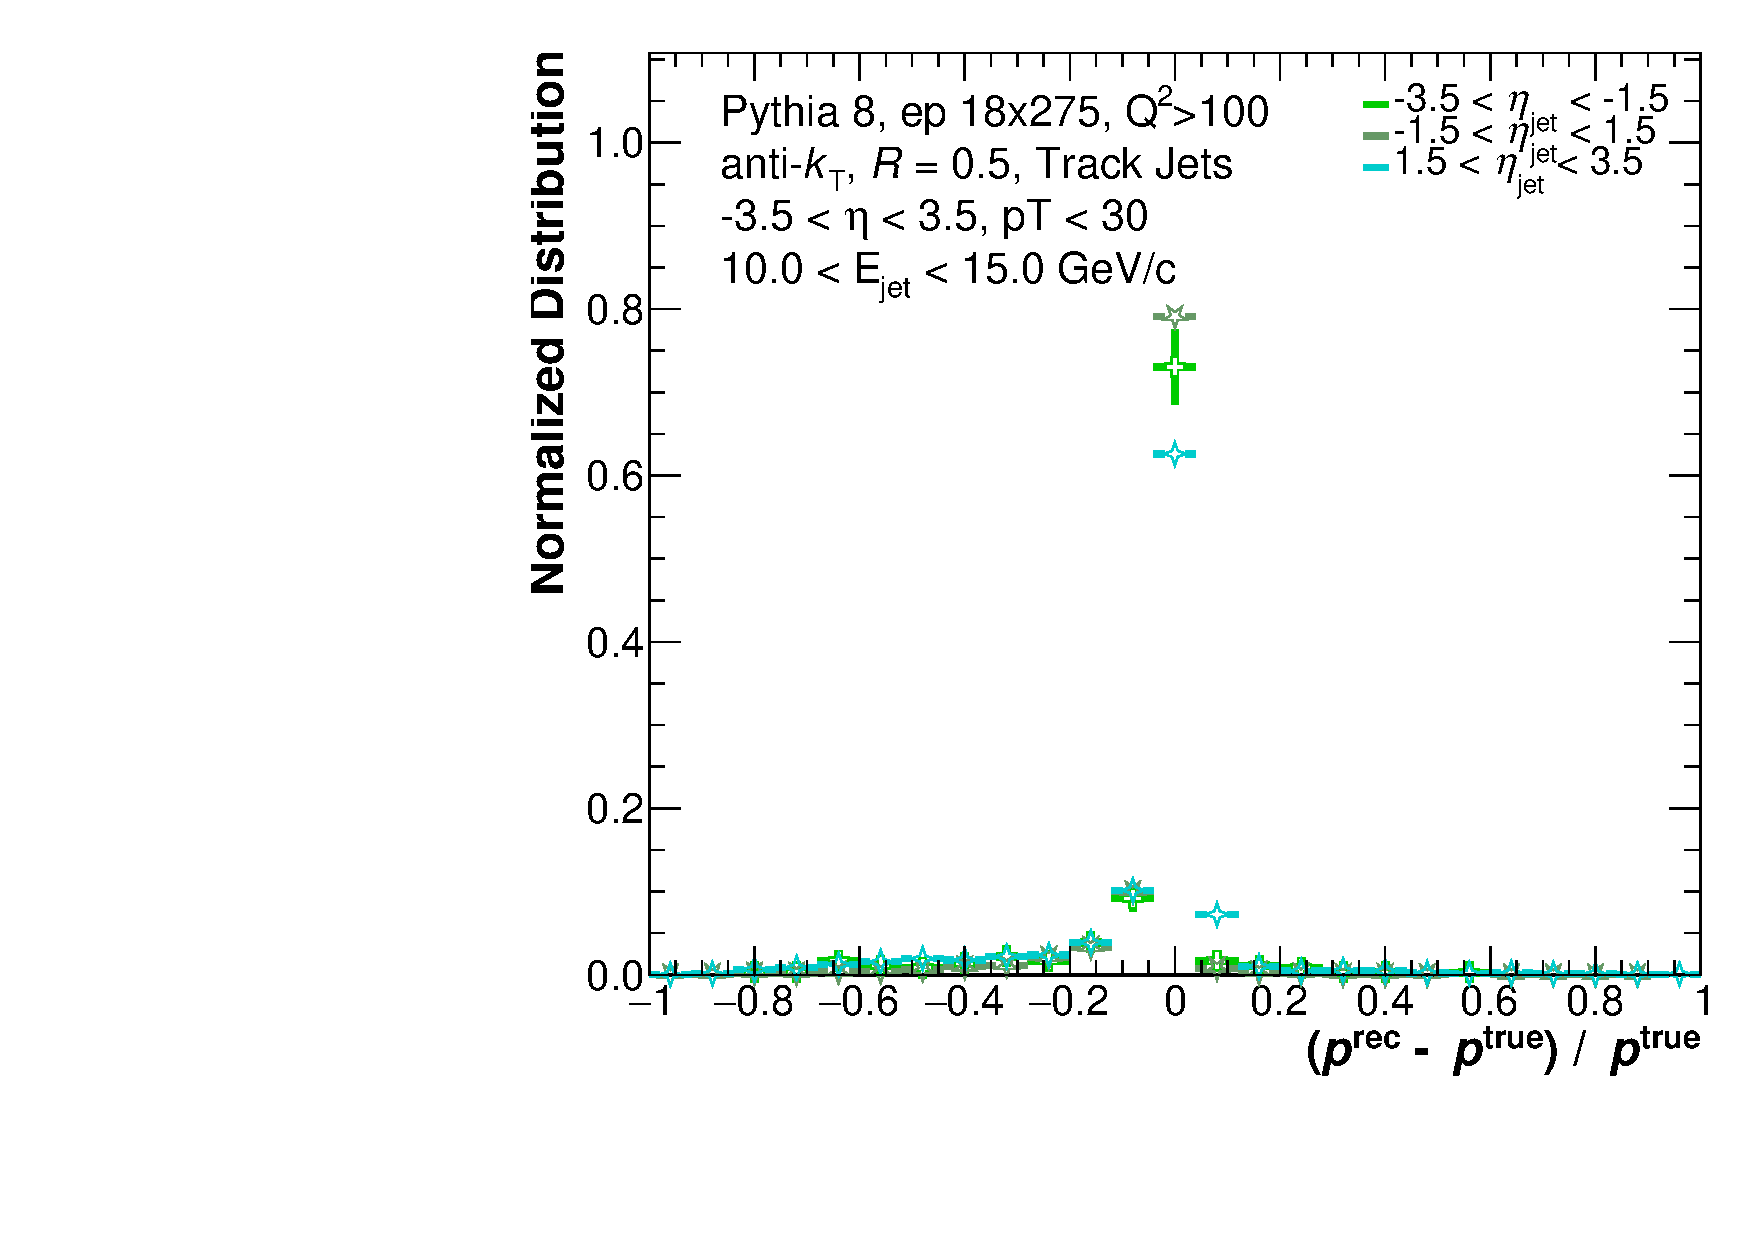
\includegraphics[width=0.6\textwidth]{figs/JES_Slice_Plot_EtaBins2_grouped.pdf}
    \caption{The distribution of the difference between the true and reconstructed momentum for track jets with a true momentum between 10 and 15 GeV/c.  The mean of the distribution determines the momentum scale of the detector, and the standard deviation of the distribution dictates the resolution.}
    \label{fig:track_momentum_slice}
\end{figure}

The scale and resolution is extracted from the distribution of 

\begin{equation}
    \frac{O^{\hbox{reconstructed}}-O^{\hbox{truth}}}{O^{\hbox{truth}}}
    \label{eq:distribution}
\end{equation}
for energy and momentum, and 
\begin{equation}
    O^{\hbox{reconstructed}}-O^{\hbox{truth}}
    \label{eq:distribution}
\end{equation}

for spatial variables, where $O$ is the observable.  From this distribution, the mean and standard deviation are calculated, corresponding to the scale and resolution respectively of the observable.  To study the response as a function of energy, the spectra was broken into 5 GeV bins, and the scale and resolution calculated for each.  An example of the 10-15 GeV/c bin for tracked jet momentum is shown in figure \ref{fig:track_momentum_slice}.




% Track jet momentum scale and resolution
\begin{figure}[h]
    \centering
    \begin{subfigure}{0.4\textwidth}
        \centering
        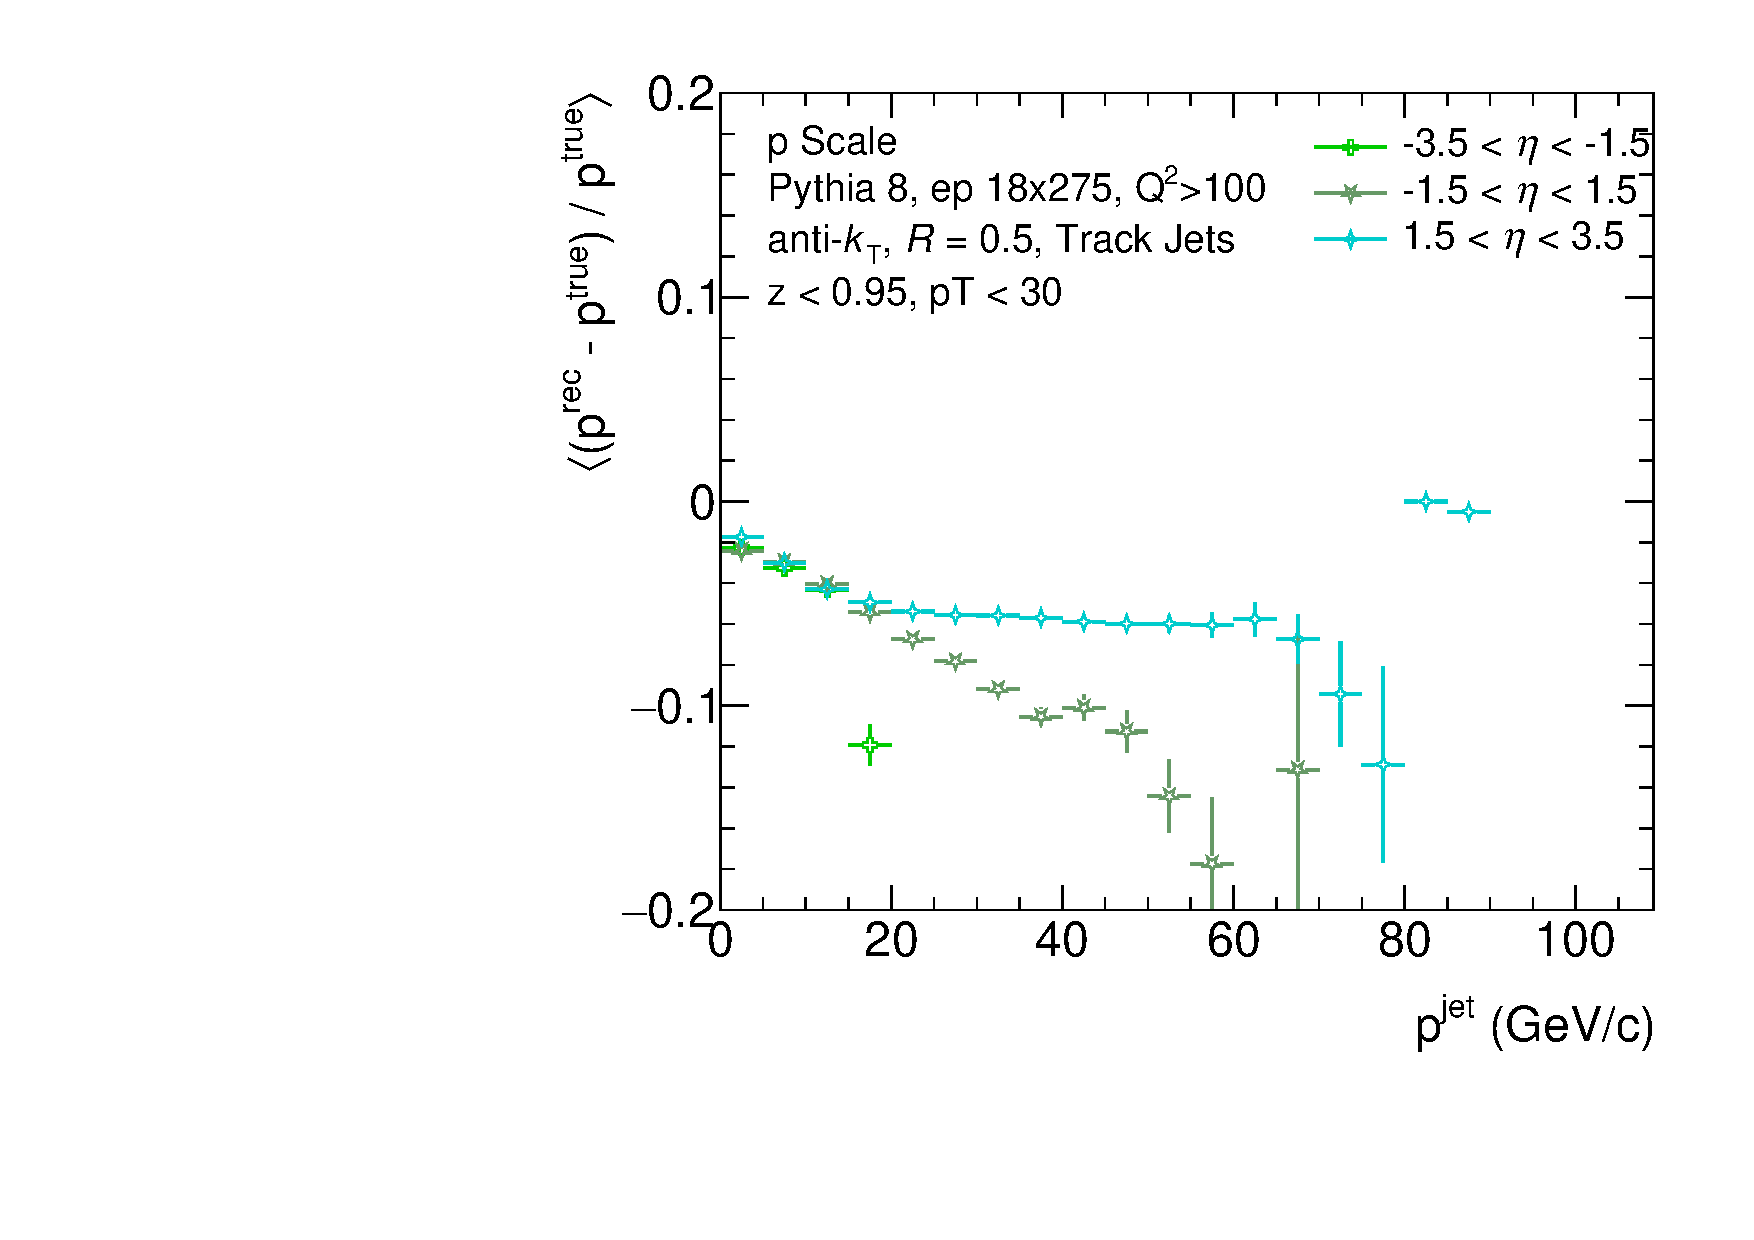
\includegraphics[width=\linewidth]{figs/Final_Plots/pScale_track_grouped.pdf}
        \caption{Track jets scale.  The scale is a measure of how much of the momentum of a truth track was reconstructed.  If all the momentum was measured, the scale would be 0, which is the ideal case.  The scale shown is still very good, and as long as it is well characterized it can be corrected for with calibrations.  }
        \label{fig:track_momentum_scale}
    \end{subfigure}
    \hfill
    \begin{subfigure}{0.4\textwidth}
        \centering
        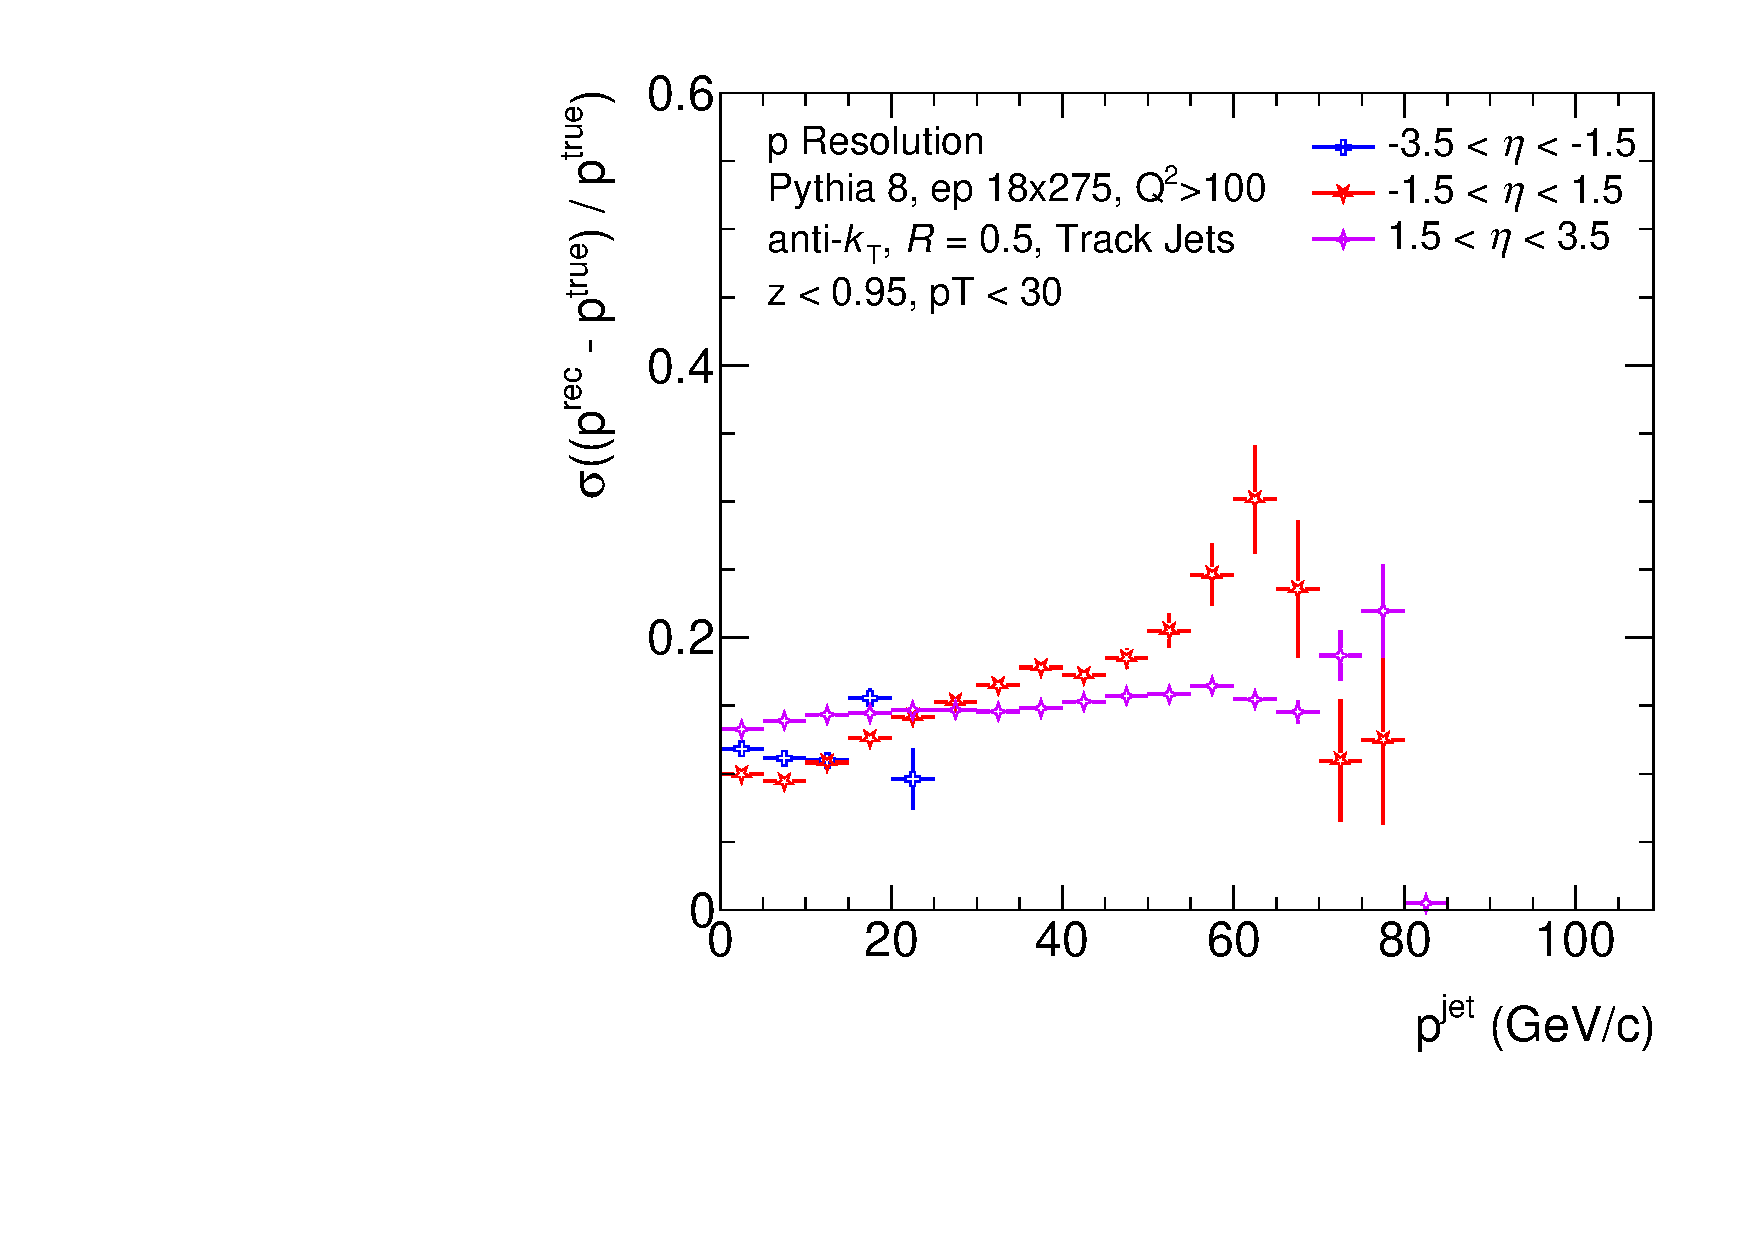
\includegraphics[width=\linewidth]{figs/Final_Plots/pReso_track_grouped.pdf}
        \caption{Track jet resolution.  The resolution is the standard deviation of the spectra of reconstructed jet momentum for a particular truth energy.  The closer the value to zero, the more confidence we have that the value is as measured.  For track jets, we anticipate the resolution to get worse as we go up in momentum, since it becomes harder for the tracking system to distinguish the momentum of the track.}
        \label{fig:track_momentum_resolution}
    \end{subfigure}
    \caption{The scale and resolution of the momentum of track jets.}
    \label{fig:track_momentum_reso_scale}
\end{figure}

As seen in figure \ref{fig:track_momentum_scale}, the jet momentum scale is better than -0.15 across entire detectors acceptance.  This, in combination with the momentum resolution better than 0.2 as shown in figure \ref{fig:track_momentum_resolution} opens up the ability to study charged jets in great detail, especially those with a momentum below 50 GeV/c.  

% Track jet spatial resolution
\begin{figure}[h]
    \centering
    \begin{subfigure}{0.4\textwidth}
        \centering
        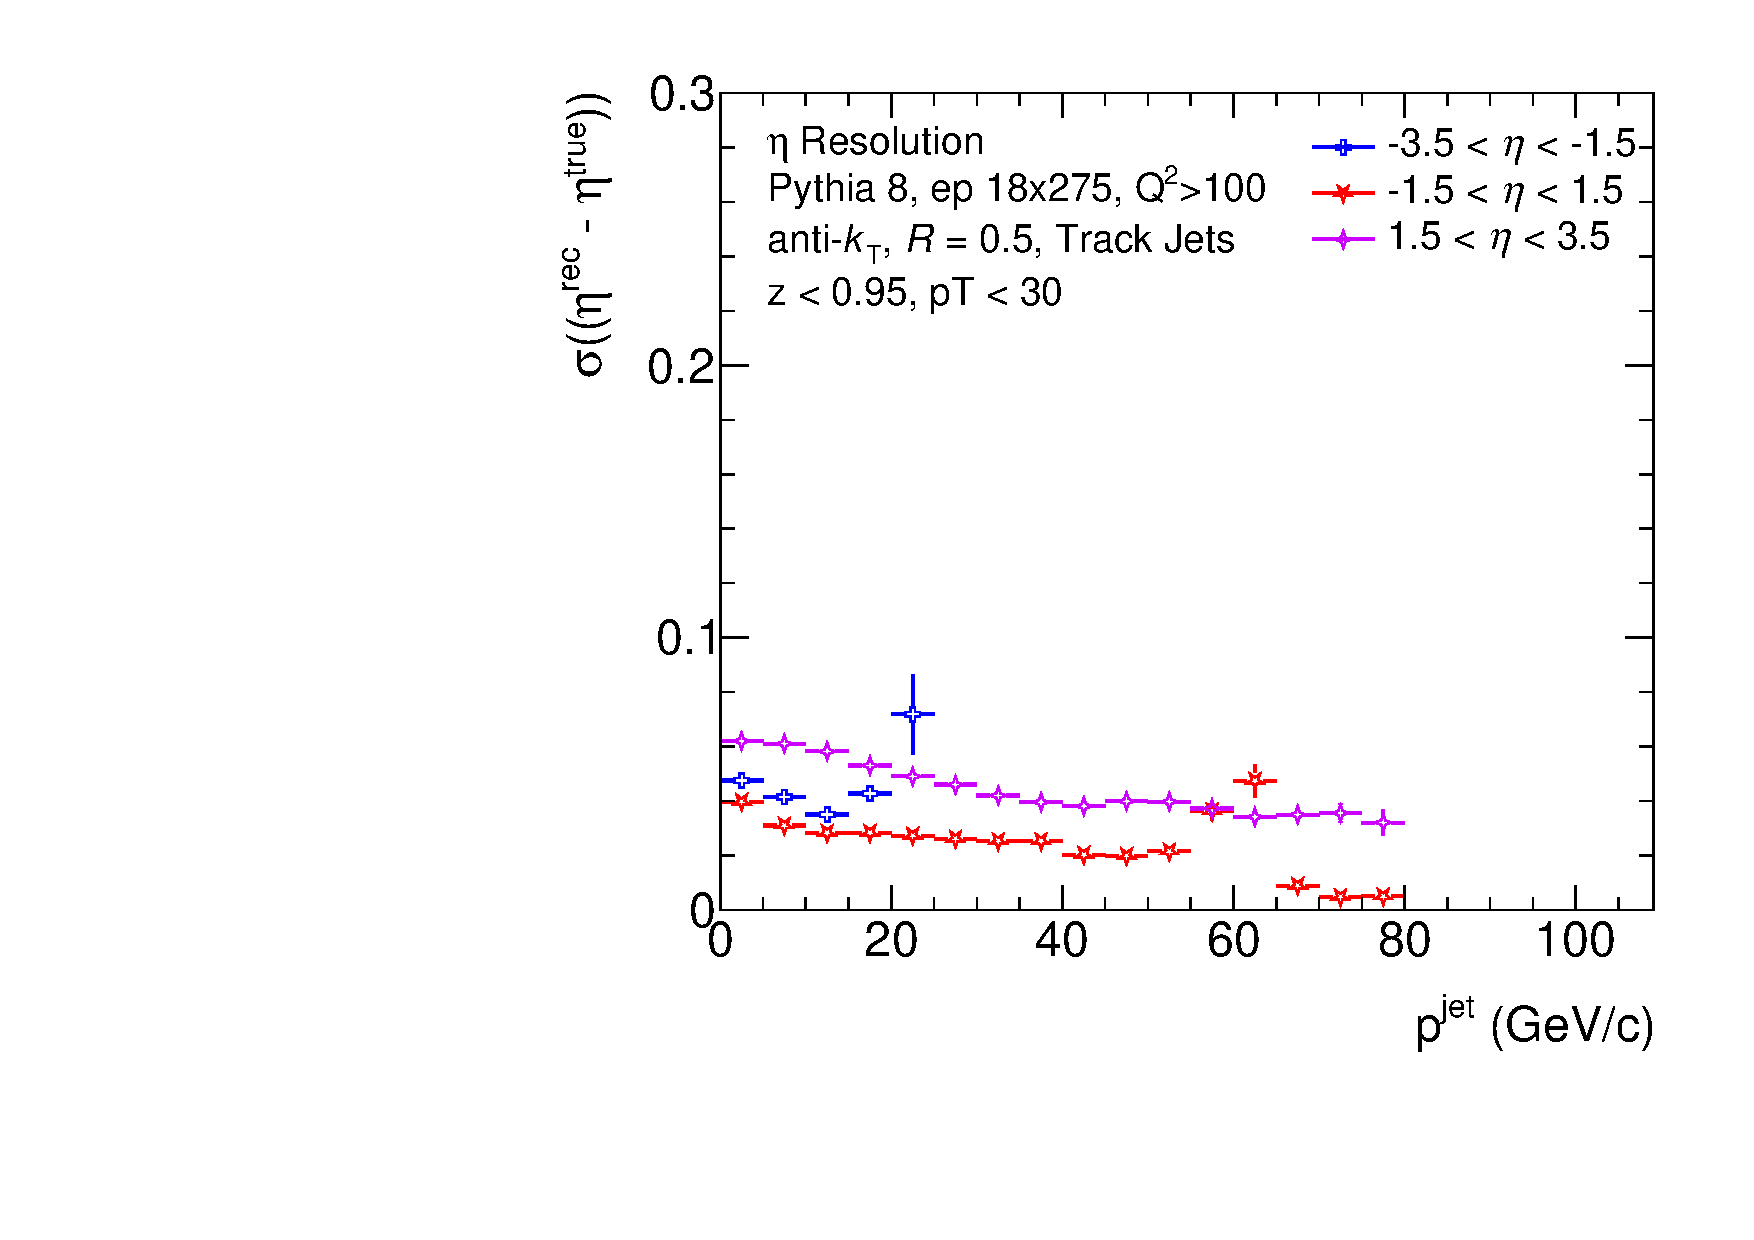
\includegraphics[width=\linewidth]{figs/Final_Plots/EtaReso_track_grouped.pdf}
        \caption{Track jet $\eta$ resolution}
        \label{fig:track_eta_resolution}
    \end{subfigure}
    \hfill
    \begin{subfigure}{0.4\textwidth}
        \centering
        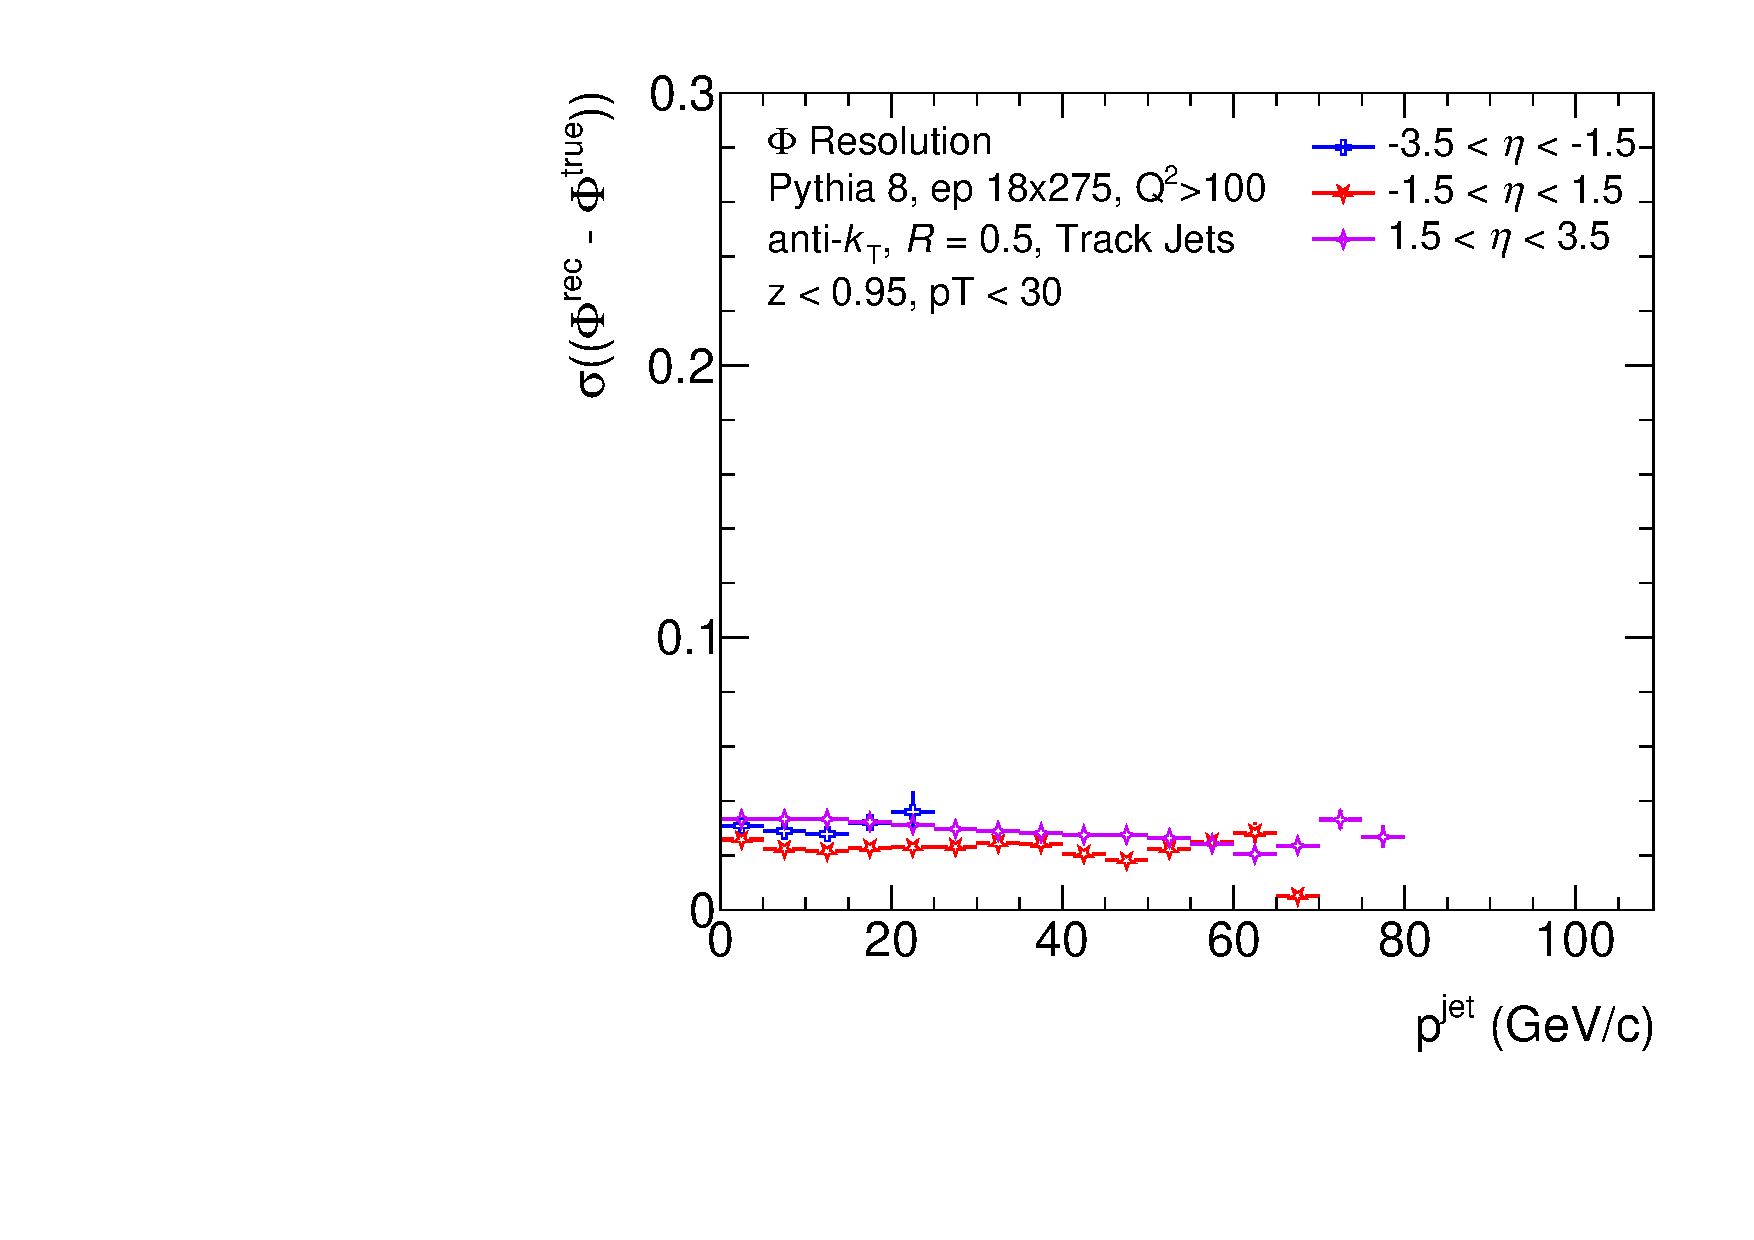
\includegraphics[width=\linewidth]{figs/Final_Plots/PhiReso_track_grouped.pdf}
        \caption{Track jet $\phi$ resolution}
        \label{fig:track_phi_resolution}
    \end{subfigure}
    \caption{The spatial resolution of track jets.  The resolution in both pseudorapidity and azimuthal angle is very good, which is important for correlating jets to the scattered electron for studying parton kinematics.  }
    \label{fig:track_spatial_reso_scale}
\end{figure}

In addition to the excellent momentum scale and resolution the ECCE tracking system offers, the detector offers very good spatial resolution of jets (Figure \ref{fig:track_spatial_reso_scale}).  \todo{this will enable the study of ...?}  

\section{Calorimetry Jets}
\label{calo_jets}

In addition to finding jets in the tracking system, ECCE's full hermetic coverage can be used to measure the energy of the charged and neutral fraction of jets.  Like in the tracking analysis, this was done with 18x275 GeV Pythia 8 electron proton collisions with a $Q^2>100\hbox{ GeV}^2$ in the prop.4 configuration.  Once again, the anti-$k_T$ jet finding algorithm was used with a jet radius $R=0.5$ with the constraint $z<0.95$.  The electromagnetic and hadronic calorimeters are used together to identify jets.

To improve the collection of energy in the calorimeters, the towers are group together with clustering algorithms to try to make each cluster contain all the energy of a single particle.  Two algorithms in particular have been utilized in this analysis, V3 and MA clustering.

V3 clustering works by starting a cluster at the most energetic tower, and adding its cardinal neighbors to it if they have less energy, but still greater than a aggregation energy parameter.  This recurses until all neighboring towers have either less energy than the aggregation energy, or greater than the current tower's energy.  The MA clustering algorithm is similar, except it will for clusters along diagonals as well as the cardinal directions.  

Both algorithms create clusters which contain the total energy accumulated among the clustered towers and has a position given by the position of each tower weighted by its energy contribution.  These clusters are then used as the input of the jet finding algorithm.  

Tuning clustering algorithms remains an ongoing process, the particular algorithms and parameters are not fixed, and may even be selected depending on the study being done. 


\begin{figure}
    \centering
    \begin{subfigure}{0.4\textwidth}
        \centering
        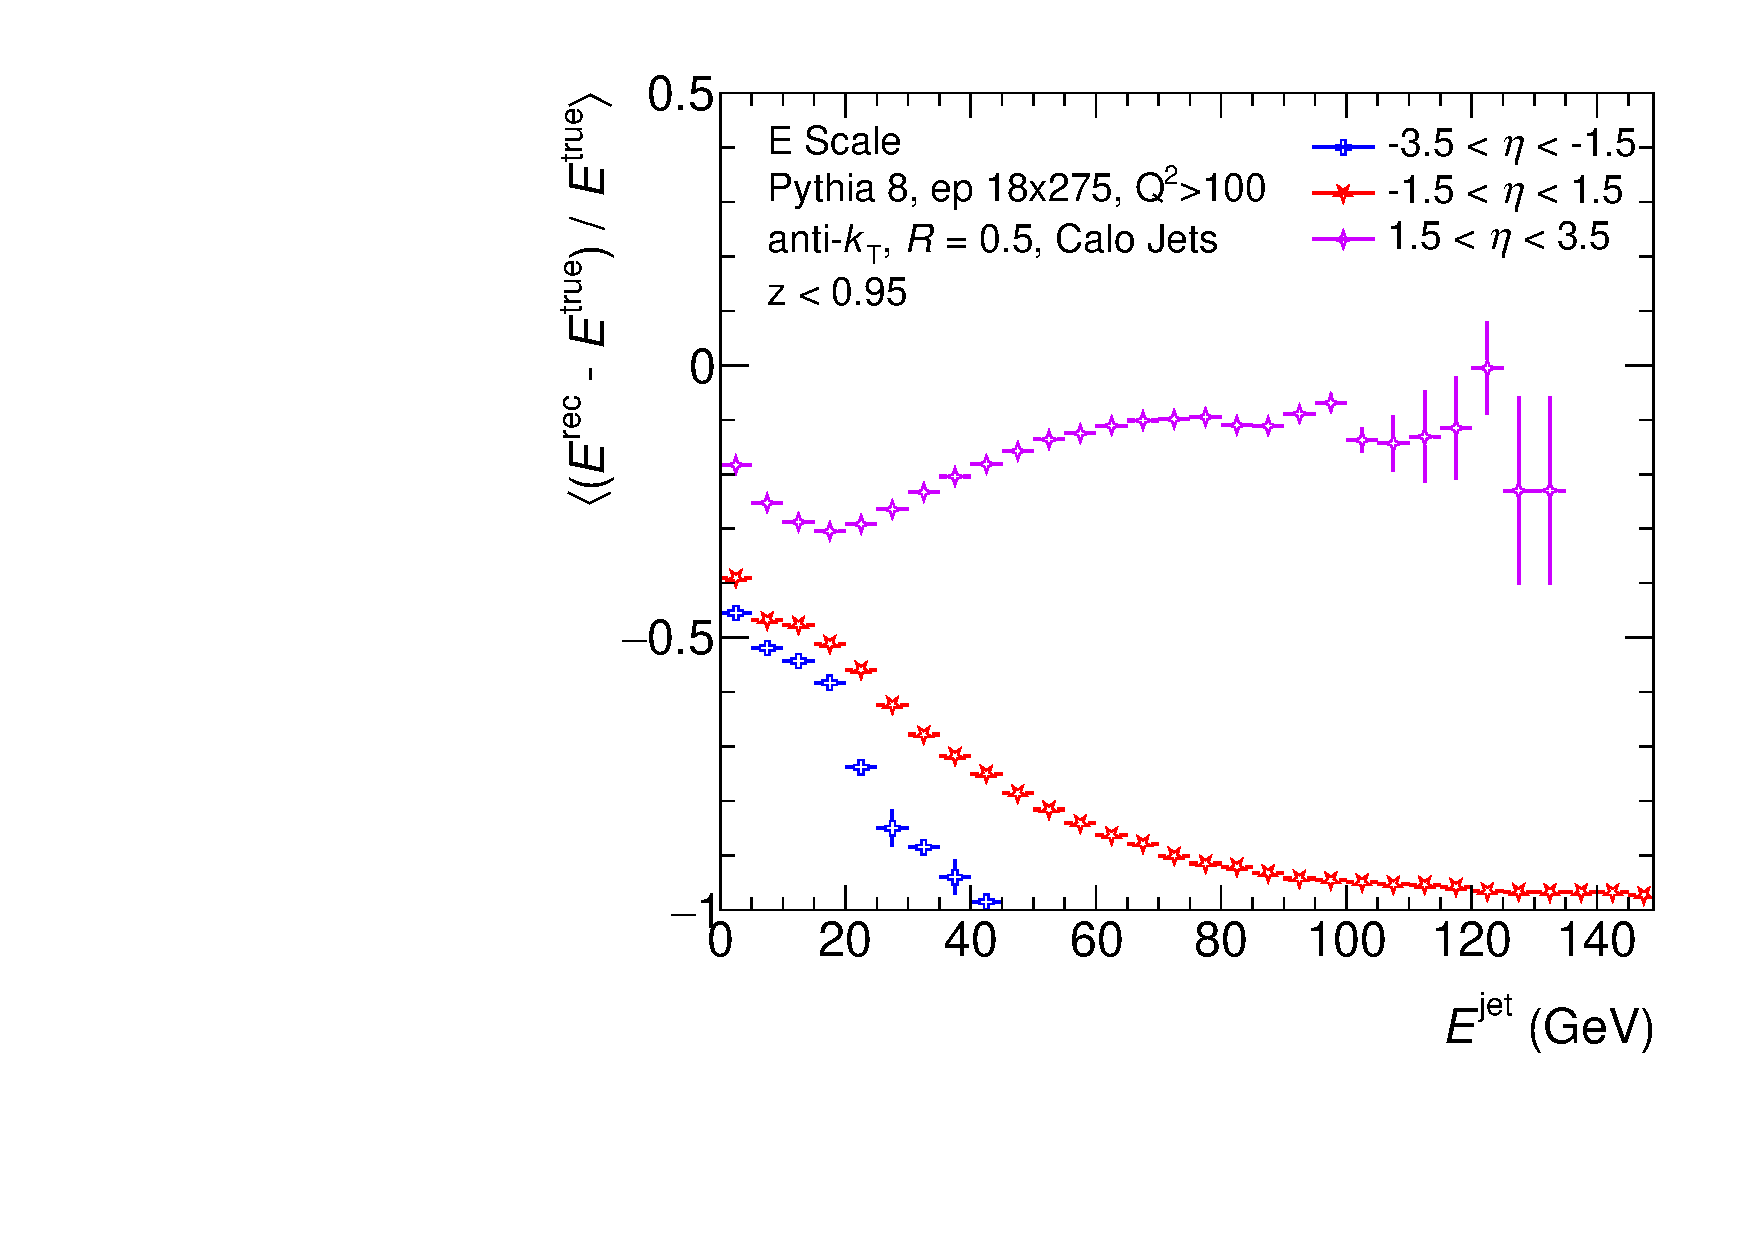
\includegraphics[width=\linewidth]{figs/Final_Plots/JES_calo_grouped.pdf}
        \caption{Calorimetry jets scale, using both hadronic and electromagnetic calorimeters.  The scale for the forward region is good, within 15\% at energies above 50 GeV.  The central and backward regions are areas where the tuning of calorimeter clustering and calibration is still ongoing, thus the poor scale.}
        \label{fig:calo_energy_scale}
    \end{subfigure}
    \hfill
    \begin{subfigure}{0.4\textwidth}
        \centering
        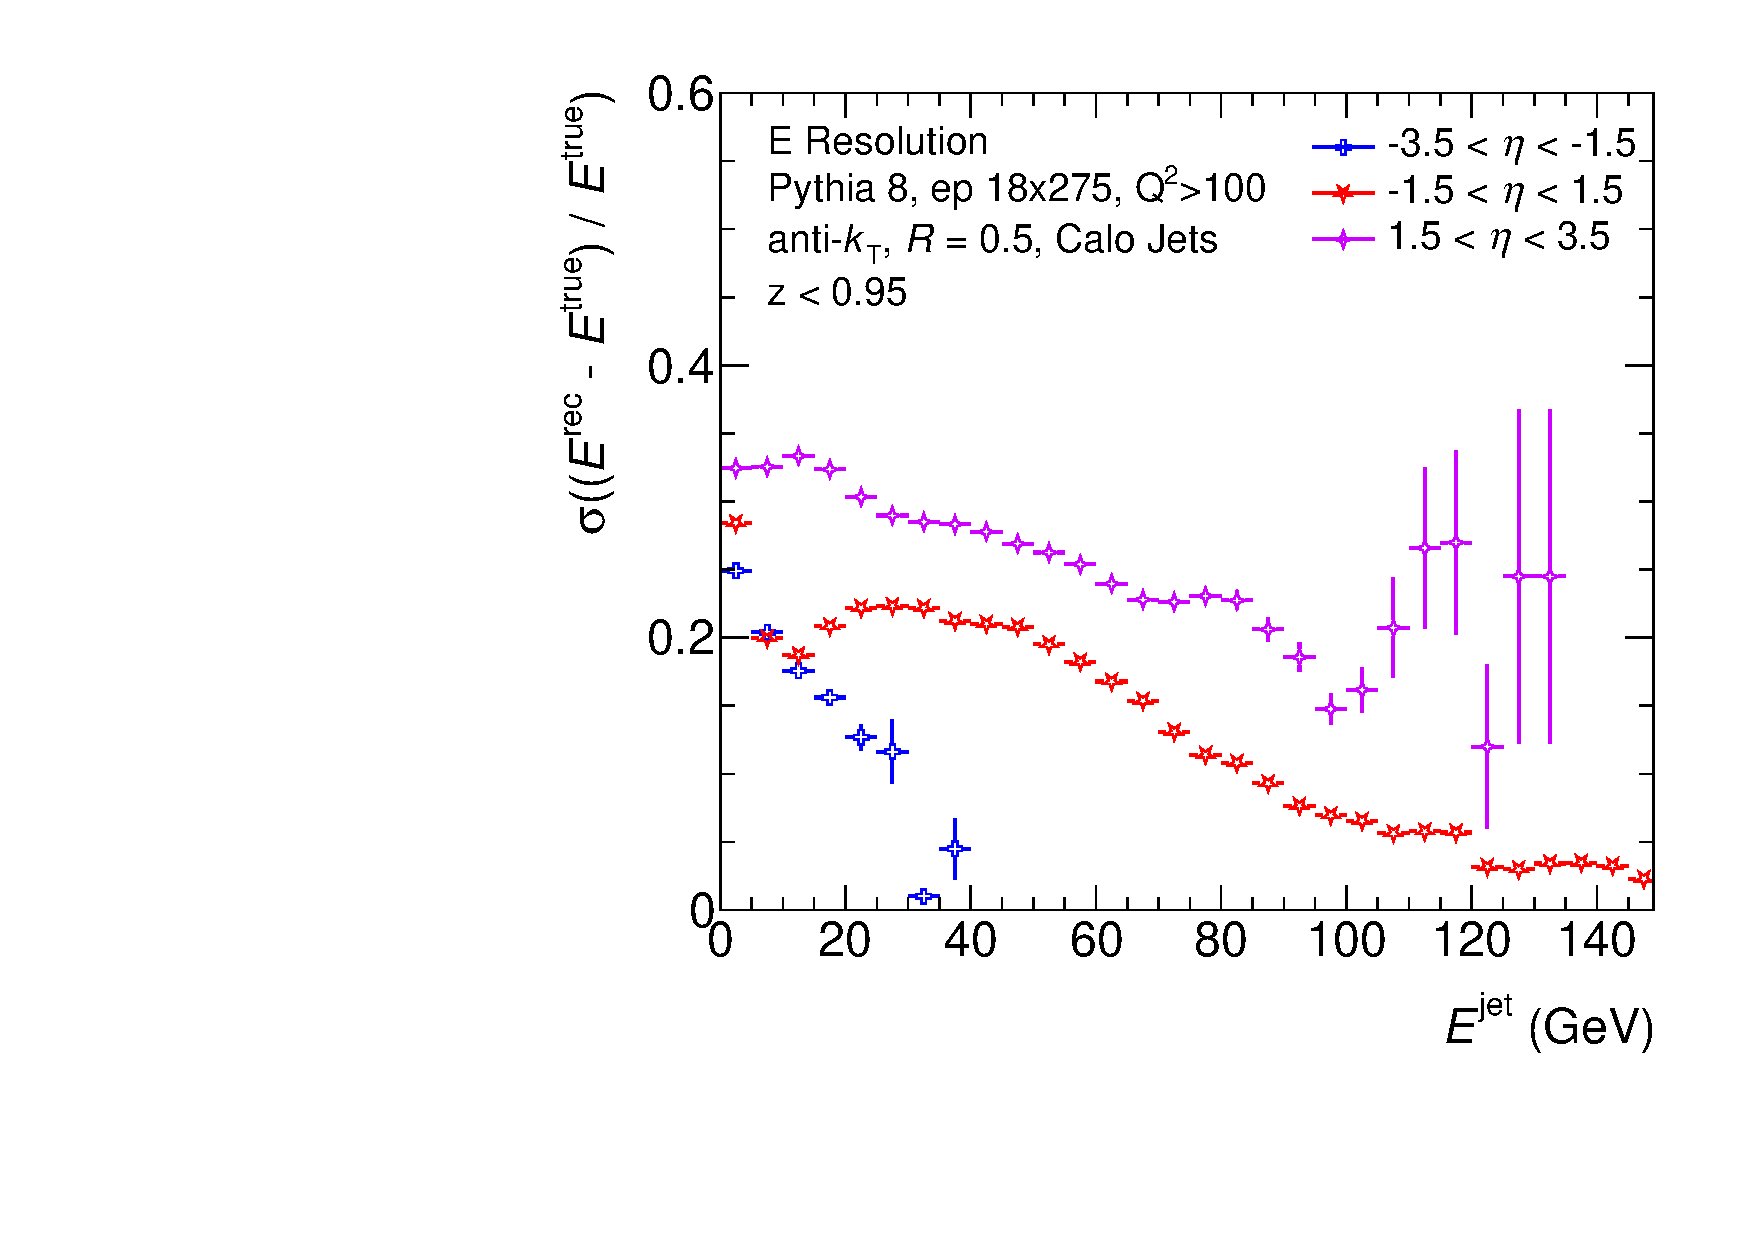
\includegraphics[width=\linewidth]{figs/Final_Plots/JER_E_calo_grouped.pdf}
        \caption{Calorimetry jet resolution.  Despite the poor scale in the central and backward region, the resolution remains good, indicating a small distribution of reconstructed energies for a particular truth energy.}
        \label{fig:calo_energy_resolution}
    \end{subfigure}
    \caption{The scale and resolution of the energy of calorimetry jets.}
    \label{fig:calo_energy_reso_scale}
\end{figure}



\begin{figure}
    \centering
    \begin{subfigure}{0.4\textwidth}
        \centering
        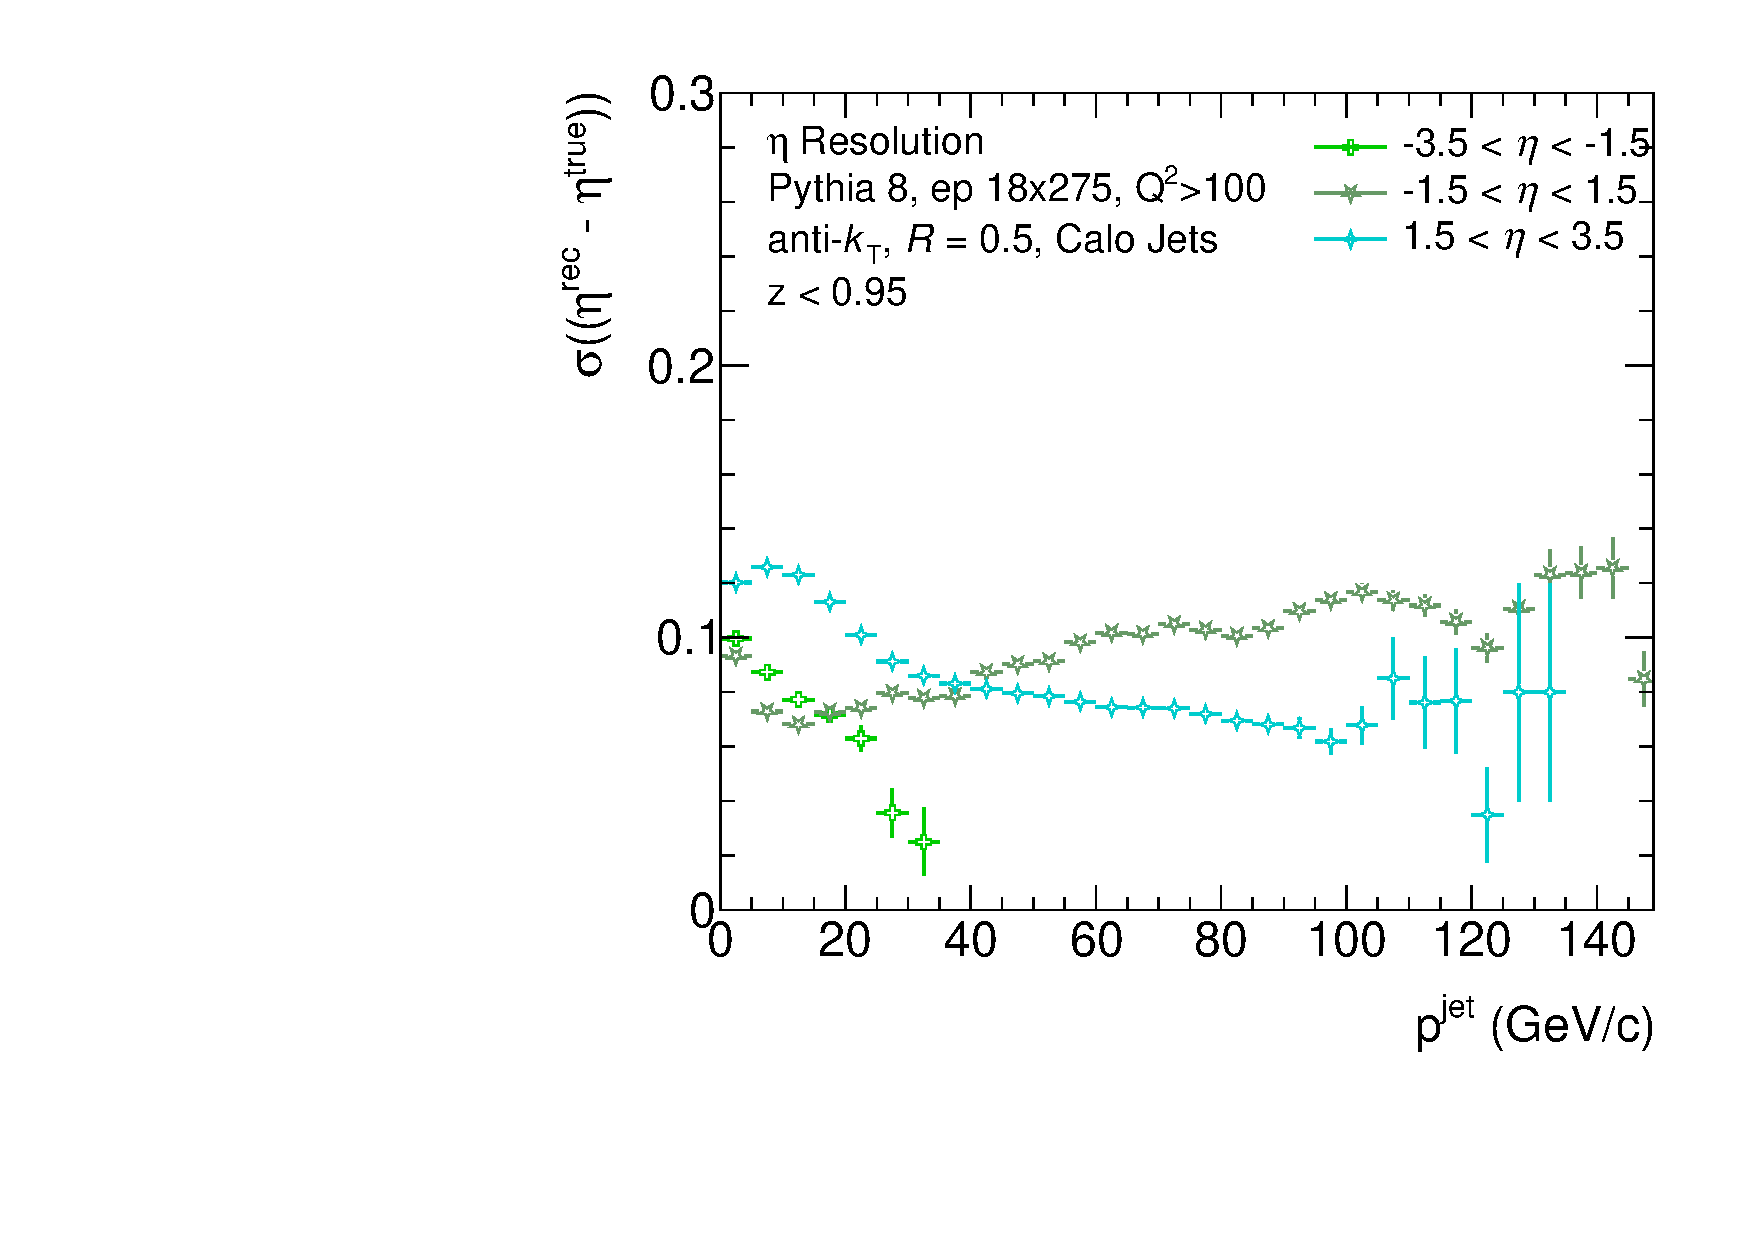
\includegraphics[width=\linewidth]{figs/Final_Plots/EtaReso_calo_grouped.pdf}
        \caption{Calorimetry jet $\eta$ resolution}
        \label{fig:calo_eta_resolution}
    \end{subfigure}
    \hfill
    \begin{subfigure}{0.4\textwidth}
        \centering
        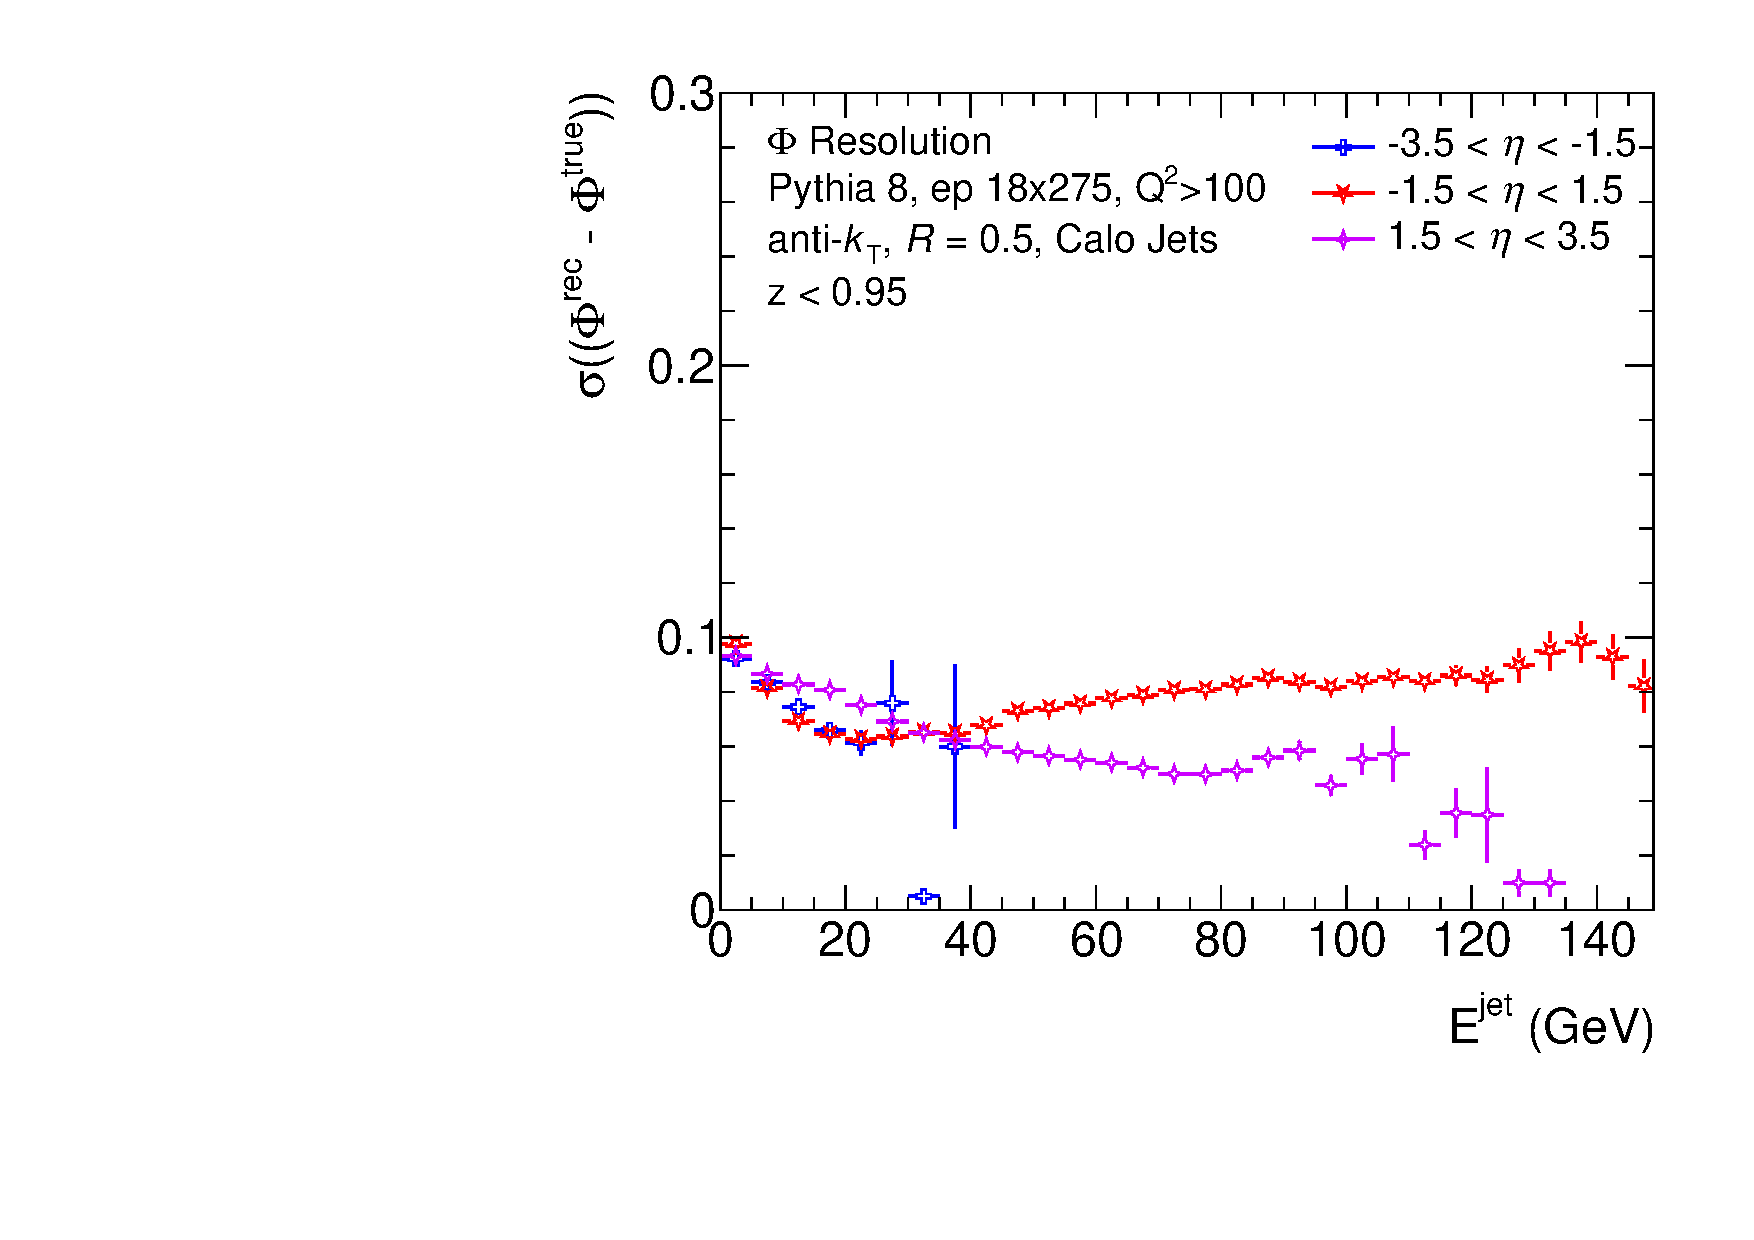
\includegraphics[width=\linewidth]{figs/Final_Plots/PhiReso_calo_grouped.pdf}
        \caption{Calorimetry jet $\phi$ resolution}
        \label{fig:calo_phi_resolution}
    \end{subfigure}
    \caption{The spatial resolution of calorimetry jets.  Since jet matching is done in $\eta-\phi$ space, the poor energy scale for the central and backward regions should have a minimal affect on the spatial resolution.}
    \label{fig:calo_spatial_reso_scale}
\end{figure}


% \listoftodos[To Do]

\bibliographystyle{unsrturl}
\bibliography{refs}

\end{document}  %%%%%%%%%%%%%%%%% End Document
